% !TeX spellcheck = de_DE
\chapter{Theoretische Grundlagen}
\label{sec:theorie}
Als schon im Abschnitt "Einleitung" erwähnt wurde, bei der Aufgabestellung es um eine Entwicklung einer Webanwendung geht. Die zu realisierende Software basiert sich, wie die meisten Webanwendungen, auf einer Client-Server-Architektur, wobei der Client Informationen eingibt, während der Server die eingegebene Daten empfängt, bearbeitet und speichert. Eine Webanwendung ist ein Computerprogramm, das eine bestimmte Funktion unter Verwendung eines Webbrowsers als Client ausführt. Die Webanwendung kann so einfach wie ein Kontaktformular auf einer Website oder so komplex wie eine Textverarbeitungs- oder Bildbearbeitungsprogramm sein, die Sie auf Ihr Computer im Browser ausführen können. Um die Webanwendung zu starten, muss der Benutzer keine zusätzlichen Programme installieren. Sie wird auf jedem Gerät mit Browser und Internetzugang ausgeführt. Der Client ist nicht vom Betriebssystem auf dem Computer des Benutzers abhängig. Bei der Entwicklung von Webanwendungen müssen daher keine separaten Versionen für Windows, Linux, Mac OS und andere Betriebssysteme geschrieben werden. Zur Implementierung der Clientseite werden HTML, CSS, JavaScript und Ajax verwendet. Zum Erstellen der Serverseite von Webanwendungen werden Programmiersprachen wie PHP, ASP, ASP.NET, Perl, C / C ++, Java, Python, Ruby und NodeJS verwendet. In dem vorherigen Schritt wurde es die Entscheidung getroffen, die Serverseite mit Web-Framework Django zu erstellen. Django wird mit einem leichten Webserver geliefert, mit dem eine  Website schnell zum Laufen gebracht werden kann, ohne Zeit mit der Einrichtung eines Servers verschwenden zu müssen. Wenn der Entwicklungsserver von Django gestartet wird, überwacht er die Codeänderungen in Echtzeit. Es wird nach dem Ändern des Codes automatisch neu geladen.

In der zu realisierenden Abschlussarbeit ist auch notwendig einen dritten Teil namens Register-Client zu entwickeln, an dem ein RFID-Leser angeschlossen wird. Der Register-Client verfügt selbst über keinen Datenbank und darf nur die abgelesene Daten dem Server schicken. Es geht um eine Simplex-Verbindung, da ein Nachrichtenverkehr asymmetrisch ist, weil der Register-Client keine Daten vom Server zurückbekommen darf und über den erfolgreiche oder gescheiterte Leihvorgang nicht wissen muss. Für die Implementierung des Register-Clients wird uComputer Raspberry Pi benutzt, der möglicherweise nicht der einzige Single-Board-Computer (SBC) auf dem Markt ist, aber bei weitem der beliebteste und schon zur Verfügung im PSE-Labor steht und ergänzend nicht geliefert werden muss. Der Raspberry Pi wird von einer großen Anzahl von Menschen verwendet und viele offizielle und inoffizielle Ressourcen und Produkte umfasst - von Büchern und Zubehör bis zu Schulungen. Dank der Raspberry Pi Foundation werden regelmäßig neue SBC-Modelle veröffentlicht. Der Raspberry Pi eignet sich aufgrund seiner hohen Rechenleistung gut als Desktop-Computer und völlig für die Verwendung in oben geschrieben Zwecken passt . 

\section{Grundlagen der Webanwendungen}
\label{sec:theorie:webapp}
In diesem Kapitel werden die grundlegenden Begriffe zum Entwerfen und Erstellen eines Webanwendung erläutert. Hierbei liegt unser Fokus nicht auf den grafischen Aspekten der Browserfunktionalität (d. H. Dem Layout von Seiten, dem Rendern von Bildern). Stattdessen konzentrieren wir uns auf die Probleme im Zusammenhang mit der Verarbeitung von HTTP-Anfragen und -Antworten. Webanwendungen können abhängig von den verschiedenen Kombinationen ihrer Hauptkomponenten in verschiedene Bestandteilen unterteilt werden. Erstens wird Das Backend (Backend oder Serverteil der Anwendung) auf einem Remotecomputer ausgeführt, der von dem Endnutzer weit entfernt werden kann oder im anliegenden Raum stehen kann.  Es ist in verschiedenen Programmiersprachen zu schrieben. Die Abschlussarbeit wird auf Python Sprache programmiert. Zweitens ist Das Frontend (Frontend oder Client-Teil der Anwendung) im Browser des Benutzers auszuführen. Die Webanwendung könnte theoretisch nur aus dem Client-Teil bestehen, wenn Benutzerdaten nicht länger als eine Sitzung gespeichert werden müssen. Dies aber ist nicht der Fall der Abschlussarbeit, da die Studentenkarten und der Verlauf des Verleihablaufs mindestens für ein laufenden Semester gespeichert werden muss, damit die Mitarbeiter des PSE-Labor immer eine Zugang zu allen gespeicherten vorherigen Leihvorgangs von der Ausleihe bis zur Rückgabe eines Boards. Es ist vorgesehen, dass am Ende des Semester nach dem letzte Rückgabe eines Boards die Datensätzen des zu Ende gegangen Semesters gelöscht wird. 

Da in den letzten Jahren sich Webanwendungen rasant weiterentwickelt und die Desktop-Lösungen schrittweise ersetzt haben und sind zu einem wesentlichen Bestandteil des Geschäfts in der modernen Welt geworden haben, es sollte auch nicht unerwähnt bleiben, welche Vorteile die Webanwendungen haben:
\begin{itemize}
	\item \textbf{Zugriff von jedem Gerät} Die Webanwendung kann überall auf der Welt von einem Computer, Tablet oder Smartphone zugegriffen und verwendet werden. Notwendig ist, dass dem Gerät eine Internetverbindung zur Verfügung steht.

\item \textbf{die Kostenersparnis} Webanwendungen können auf allen Plattformen ausgeführt werden und müssen nicht mehr separat für Android und iOS entwickelt werden.

\item \textbf{Anpassungsfähigkeit} Wenn native Anwendungen bestimmte Betriebssysteme erfordern, jedoch können jedes Betriebssystem (Windows, MAC, Linux usw.) und jeder Browser (Internet Explorer, Opera, FireFox, Google Chrome usw.) für die Arbeit mit einer Webanwendung. ) verwendet werden.

\item \textbf{Keine Software zum Herunterladen} Es ist günstig und einfach dem Endnutzer zu liefern, zu warten und zu aktualisieren. Das Aktualisieren auf die neueste Version erfolgt beim nächsten Laden der Webseite.

\item \textbf{Netzwerksicherheit} Das Websystem verfügt über einen einzigen Einstiegspunkt, der zentral geschützt und konfiguriert werden kann.

\item \textbf{Skalierbarkeit} Mit zunehmender Belastung des Systems ist es nicht erforderlich, die Leistung des Computer von Endbenutzer zu erhöhen. Mit einer Webanwendung kann in der Regel nur mithilfe von Hardwareressourcen eine größere Datenmenge verarbeitet werden, ohne den Quellcode neu zu schreiben und die Architektur ändern zu müssen.

\item \textbf{Verhinderung von Datenverlust} Benutzerdaten werden in der "Cloud" gespeichert, für deren Integrität die Hosting-Anbieter verantwortlich sind, deswegen vom Verlust geschützt, falls die Festplatte des Computers beschädigt wird.
\end{itemize}

Als nächstes geht die Frage nach, wie Client und Server miteinander kommunizieren können. Der Client spricht mit dem Server über \hyperref[sec:appendix:http]{das HTTP-Protokoll}. Das HTTP-Protokoll setzt die Verwendung einer Client-Server-Datenübertragungsstruktur voraus. Die Clientanwendung generiert eine Anforderung und sendet sie an den Server. Anschließend verarbeitet die Serversoftware diese Anforderung, generiert eine Antwort und sendet sie an den Client zurück. Die Clientanwendung kann dann weiterhin andere Anforderungen senden, die auf ähnliche Weise behandelt werden. Wenn ein Webserver eine Anforderung zum Bereitstellen einer statischen Webseite erhält, sendet er die Seite direkt an den Browser.\cite{website:2} Wenn jedoch eine dynamische Seite angefordert wird, sind die Handlungsweise des Webservers nicht so einfach. Der Server übergibt die Seite an ein spezielles Programm, das die letzte Seite bildet. Ein solches Programm wird als Anwendungsserver bezeichnet. Der Anwendungsserver liest den Code auf der Seite, rendert die letzte Seite gemäß dem gelesenen Code und entfernt sie dann von der Seite. Als Ergebnis all dieser Operationen wird eine statische Seite erhalten, die an den Webserver übertragen wird, der sie wiederum an den Client-Browser sendet. Alle Seiten, die der Browser empfängt, enthalten nur HTML-Code.\cite{website:2} Schematische Darstellung des Prozesses kann man auf der Abbildung \ref{fig:client-server}\cite{website:2} ansehen. Die Anforderung kann mit den GET-Methoden erfolgen, wenn wir Daten empfangen möchten, und mit POST, wenn wir die Daten ändern möchten. Die Anfrage enthält auch den Host (Site-Domain), den Anfragetext (wenn es sich um eine POST-Anfrage handelt) und viele zusätzliche technische Informationen. 
\begin{wrapfigure}{l}{0.55\textwidth}
	\fbox{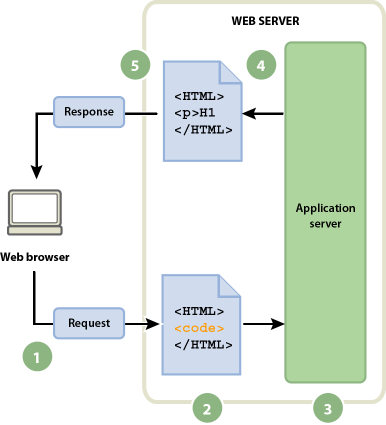
\includegraphics[width=0.52\textwidth]{gfx/ds_process_dynamic.png}}
	\caption{Schematische Darstellung der Client-Server Kommunikation}
	\label{fig:client-server}
\end{wrapfigure}
 Das HTTP-Protokoll ist ein zustandsloses Protokoll auf Anwendungsebene und bietet keine Speicherung von Informationen über die Sitzung des Benutzers; jede Datenübertragung wird als neue Sitzung betrachtet. Da HTTP per Definition ein zustandsloses Protokoll ist, wurde es nicht für die Unterstützung dauerhafter Verbindungen entwickelt. Eine Verbindung sollte lange genug dauern, damit ein Browser eine Anfrage senden und eine Antwort erhalten kann. Eine Verlängerung der Lebensdauer einer Anfrage darüber hinaus wurde nicht unterstützt.\cite[p.62]{shklar:webapplication} 

Am Rande sei auch eine weitere Technologie erwähnt, die uns ständig begegnet. Cache (Cache) ist ein Konzept in der Entwicklung, bei dem häufig verwendete Daten, anstatt jedes Mal aus der Datenbank abgerufen, berechnet oder auf andere Weise vorbereitet, an einem schnell zugänglichen Ort gespeichert werden. Einige Beispiele für die Verwendung des Caches:
\begin{itemize}
	\item Django erhielt eine Anfrage, Daten für ein Diagramm in einem Bericht abzurufen. Daten aus der Datenbank werden abgeholt, vorbereitet und abgelegt in einer Datenbank mit schnellem Zugriff z.B. "memcached", die beispielsweise für eine Stunde zwischengespeichert wird. Bei der nächsten Anfrage werden die notwendigen Daten sofort von "memcached" erhalten und an das Frontend gesendet. Wenn es festgestellt wird, dass die Daten nicht mehr relevant sind, werden sie ungültig beziehungsweise gelöscht aus dem Cache.

	\item CDN-Anbieter (Content Delivery Network) werden zum Zwischenspeichern statischer Dateien verwendet. Hierbei handelt es sich um Servers auf der ganzen Welt, die für die Bereitstellung statischer Inhalte optimiert sind. Manchmal ist es effizienter, Bilder, Videos und JS-Skripte auf einem CDN anstatt auf Ihrem eigenen Server abzulegen.

	\item In allen Browsern ist das statische Zwischenspeichern von Dateien standardmäßig aktiviert. Da die Website nicht zum ersten Mal geöffnet wird, werden die dazugehörige Daten aus dem Zwischenspeichern viel schneller geladen. Der Nachteil für den Entwickler ist, dass bei aktiviertem Cache die vorgenommenen Änderungen nicht immer sofort sichtbar sind. 
\end{itemize}

Daraus lässt sich die Schlussfolgerung ziehen, dass eine Webanwendung für einen Endnutzer wie eine Website aussieht, auf der  die Webseiten mit teilweise oder vollständig nicht formatiertem Inhalt sich befinden. Die Endfertigung des Inhalts findet nur dann statt, nachdem ein Website-Besucher die Seite vom Webserver angefordert hat. 

In diesem Kapitel wurden die Grundlagen der Webanwendungen und des HTTP-Protokolls erörtert. Diese Diskussion war nicht als umfassende Beschreibung aller Funktionen gedacht, eher als Überblick über das Verständnis und die Arbeit mit aktuellen Stand der Technologie und zukünftigen Verwendung der entwickelte Software im PSE-Labor. 

\section{Raspberry Pi Board und OS}
\label{sec:theorie:raspberry}
\begin{wrapfigure}{l}{0.48\textwidth}
	\fbox{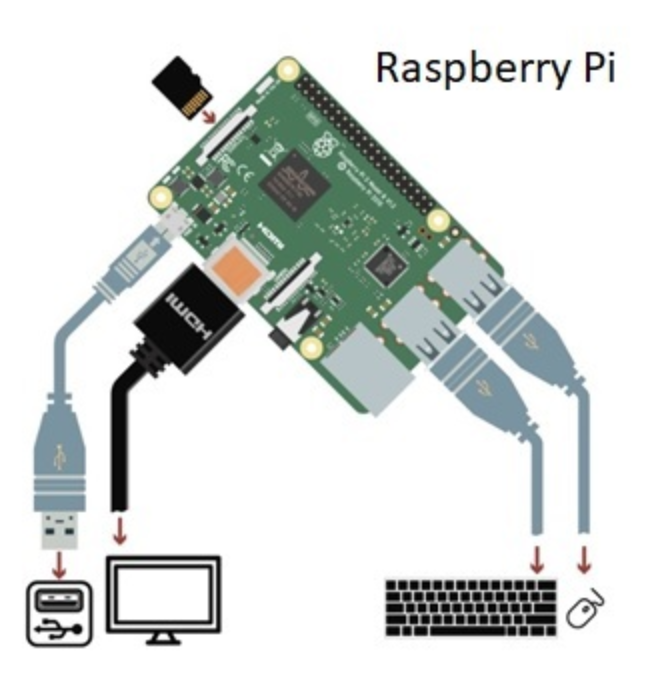
\includegraphics[width=0.45\textwidth]{gfx/rasp.png}}
	\caption{Peripherieanschlüsse der Raspberry Pi}
	\label{fig:rasp}
\end{wrapfigure}
Raspberry Pi ist ein Einplatinencomputer, wobei die verschiedene Teile des Computers, die sich normalerweise auf separaten Platinen befinden, werden hier nur auf einer dargestellt. Darüber hinaus hat diese Platte eine relativ kleine Größe - ungefähr 8,5 * 5,5 cm.mDer Produktname kombiniert Raspberry-Himbeer- und Pi- die Kraiszahl Pi. Das Himbeerbild wurde zum Logo des Projekts. Der Raspberry Pi ist eine kostengünstige Plattform - sein empfohlener Verkaufspreis beträgt weniger als 50€. Ein Mikrocomputer verfügt über alle Funktionen eines Personal Computer (PC): Prozessor, Speicher, Betriebssystem, Anschluss an einen Monitor (TV), die Vernetzung. Der Raspberry Pi verfügt im Gegensatz zu einem PC über zusätzliche Peripheriegeräte wie GPIO-Ports (General Purpose Input / Output). Über diese Pins kann der Mikrocomputer mit der elektronischen Welt der Sensoren, Bildschirmen und Aktoren interagieren. In Abbildung \ref{fig:rasp}\cite{website:3} sind die Anschlüsse schematisch dargestellt.
\section{Kontaktlose Chipkartentechnik MIFARE}
\label{sec:theorie:mifare}

\section{Sender-Empfänger-System mit RFID}
\label{sec:theorie:rfid}

\section{Datenbanken mit Python und SQLite}
\label{sec:theorie:db}

\section{HTTP für Design der verteilten Systeme}
\label{sec:theorie:http}

\section{Django Framework}
\label{sec:theorie:about_django}

\section{API}
\label{sec:theorie:api}

\section{Endliche Zustandsmaschine}
\label{sec:theorie:fsm}

\section{Clientseitiges JavaScript}
\label{sec:theorie:js}




